\documentclass[12pt,a4paper]{ctexart}
\usepackage[utf8]{inputenc}
\usepackage{easyReview}
\usepackage[T1]{fontenc}
\usepackage{amsmath}
\usepackage{fancyhdr}
\usepackage{amsfonts}
\usepackage{booktabs}
\usepackage{subcaption}
\usepackage{float}
\usepackage{mathrsfs}
\usepackage{bm}
\usepackage{extarrows}
\usepackage{wasysym}
\usepackage{graphbox}
\usepackage{graphicx}
\usepackage[colorlinks,linkcolor=red,anchorcolor=blue,citecolor=green]{hyperref}
\usepackage{cases}
\usepackage{color}
\usepackage{tcolorbox}
\usepackage{listings}
\usepackage{xcolor}
\usepackage[framemethod=tikz]{mdframed}
\usepackage[left=2.00cm, right=2.00cm, top=2.00cm, bottom=2.00cm]{geometry}

\newcommand{\RNum}[1]{\uppercase\expandafter{\romannumeral #1\relax}}
\newtheorem{theorem}{定理}[section]
\newtheorem{lemma}[theorem]{Lemma}
\newtheorem{definition}[theorem]{定义}
\newtheorem{example}[theorem]{例}
\newtheorem{exercise}[theorem]{\textcolor{blue} {练习}}
\newtheorem{problem}[theorem]{问题}
\newtheorem{property}[theorem]{性质}
\newtheorem{proposition}[theorem]{命题}
\newtheorem{remark}[theorem]{Remark}
\newtheorem{algorithm}[theorem]{算法}

\pagestyle{fancy}
\cfoot{\thepage}
\lhead{{《最优化理论与方法》实验报告}}
\setlength{\headheight}{14.5pt}

\lstset{
    language=Python,
    basicstyle=\ttfamily\small,
    keywordstyle=\color{blue!70!black},
    commentstyle=\color{green!40!black},
    stringstyle=\color{red!60!black},
    numbers=left,
    numberstyle=\tiny\color{gray},
    stepnumber=1,
    frame=single,
    breaklines=true,
    showstringspaces=false,
    tabsize=4
}

\begin{document}

\vspace*{6em}
\begin{figure}[H]
	\centering
	
\includegraphics[width=0.4\linewidth]{picture/HNUlogo}
\end{figure}
\vspace*{4em}
\begin{center}
{\Huge \bf 《最优化算法与理论》实验报告}
\end{center}
\vspace{4em}
\begin{center}
{\Large
{\bf\makebox[4em][s]{实验序号}}: \underline{\makebox[13em][c]{3}}\\
{\bf\makebox[4em][s]{实验内容}}: \underline{\makebox[13em][c]{BB步长、拟牛顿法与共轭梯度法}}\\
{\bf\makebox[4em][s]{班~~~~级}}: \underline{\makebox[13em][c]{信息2301}}\\
{\bf\makebox[4em][s]{学~~~~号}}: \underline{\makebox[13em][c]{202310040128}}\\
{\bf\makebox[4em][s]{姓~~~~名}}: \underline{\makebox[13em][c]{雷龙浩}}\\
{\bf\makebox[4em][s]{完成日期}}: \underline{\makebox[13em][c]{2026年03月31日}}\\
}
\end{center}
\clearpage

\tableofcontents
\newpage

\section{实验任务与实现说明}
本次上机练习的两项核心任务如下：
\begin{itemize}
  \item 实现采用 BB 步长的最速下降法，求解 Rosenbrock 函数极小化问题；
  \item 采用 Armijo 回溯步长搜索，实现 BFGS（代码中函数名为 \texttt{bfgc}）与 FR 共轭梯度法（\texttt{fr}），求解 Powell 奇异函数。
\end{itemize}

实验代码入口为 \texttt{work3/work3.py}，运行命令为：
\begin{quote}
\texttt{python work3/work3.py}
\end{quote}
脚本会自动输出结果表，并在 \texttt{work3/picture/} 下生成收敛曲线与轨迹图。

\subsection{算法原理简述}
\textbf{1) BB 步长思想}

对于最速下降法迭代
\[
x_{k+1}=x_k-\alpha_k \nabla f(x_k),
\]
BB 方法通过两点信息近似曲率，定义
\[
s_k=x_k-x_{k-1},\qquad y_k=\nabla f(x_k)-\nabla f(x_{k-1}),
\]
并用
\[
\alpha_k^{\text{BB1}}=\frac{s_k^Ts_k}{s_k^Ty_k},\qquad
\alpha_k^{\text{BB2}}=\frac{s_k^Ty_k}{y_k^Ty_k}
\]
给出步长候选。本实验代码中默认采用 \texttt{auto} 策略，在正值候选里取更保守值。

\textbf{2) Armijo 回溯条件}
\[
f(x_k+\alpha d_k)\le f(x_k)+\sigma_1\alpha \nabla f(x_k)^Td_k,\quad
0<\sigma_1<0.5.
\]
若条件不满足，则执行 \(\alpha\leftarrow \rho\alpha\)（\(0<\rho<1\)）回溯缩步。

\textbf{3) BFGS 与 FR}
\[
B_k d_k=-g_k,\qquad
B_{k+1}=B_k-\frac{B_ks_ks_k^TB_k}{s_k^TB_ks_k}+\frac{y_ky_k^T}{y_k^Ts_k}.
\]
FR 共轭梯度法使用
\[
\beta_k^{\text{FR}}=\frac{g_{k+1}^Tg_{k+1}}{g_k^Tg_k},\qquad
d_{k+1}=-g_{k+1}+\beta_k^{\text{FR}}d_k.
\]

\subsection{程序结构与关键代码}
本次实验采用“目标函数定义 + 优化器 + 步长搜索 + 实验脚本”分层结构。核心文件如下：
\begin{itemize}
  \item \texttt{work3/work3.py}：组织实验、绘图、输出表格；
  \item \texttt{optimization/line\_search/bb.py}：BB 步长实现；
  \item \texttt{optimization/optimizers/BFGC.py}：BFGS 优化器实现；
  \item \texttt{optimization/optimizers/FR.py}：FR 共轭梯度实现。
\end{itemize}

\textbf{代码展示 1：work3 主实验流程（两组实验）}
\lstinputlisting[
    firstline=182,
    lastline=260,
    caption={work3.py 中实验主流程与参数配置},
    label={lst:work3-main}
]{work3.py}

\textbf{代码展示 2：BB 步长搜索实现}
\begin{lstlisting}[caption={BB 步长计算核心代码},label={lst:bb-impl}]
def bb_step_search(
    xk: np.ndarray,
    _dk: np.ndarray,
    objective: Objective,
    x_prev: np.ndarray | None = None,
    alpha_init: float = 0.1,
    variant: str = "auto",
    eps: float = 1e-12,
    **_: object,
) -> Tuple[float, int]:
    if x_prev is None:
        return float(alpha_init), 0

    xk = np.asarray(xk, dtype=float)
    x_prev = np.asarray(x_prev, dtype=float)
    sk = xk - x_prev
    yk = objective.gradient(xk) - objective.gradient(x_prev)

    sTy = float(np.dot(sk, yk))
    sTs = float(np.dot(sk, sk))
    yTy = float(np.dot(yk, yk))

    alpha_bb1 = None
    alpha_bb2 = None
    if abs(sTy) > eps:
        alpha_bb1 = sTs / sTy
    if yTy > eps:
        alpha_bb2 = sTy / yTy

    variant_key = variant.strip().lower()
    if variant_key == "bb1":
        alpha = alpha_bb1
    elif variant_key == "bb2":
        alpha = alpha_bb2
    elif variant_key == "auto":
        candidates = [a for a in (alpha_bb1, alpha_bb2) if a is not None and a > 0.0]
        alpha = min(candidates) if candidates else None
    else:
        raise ValueError("variant must be one of {'bb1', 'bb2', 'auto'}.")

    if alpha is None or (not np.isfinite(alpha)) or alpha <= 0.0:
        alpha = alpha_init

    return float(alpha), 0
\end{lstlisting}

\textbf{代码展示 3：BFGC 与 FR 算法核心迭代}
\begin{lstlisting}[caption={BFGC.py 中 BFGS 主迭代代码},label={lst:bfgc-impl}]
def bfgc(
    x0: np.ndarray,
    objective: Objective,
    line_search_func: LineSearch = wolfe_powell_line_search,
    grad_tol: float = 1e-6,
    max_outer_iter: int = 1000,
    callback: Optional[IterationCallback] = None,
    **ls_params,
) -> Tuple[np.ndarray, float, int, bool, float]:
    xk = np.asarray(x0, dtype=float)
    n = xk.size
    bk = np.eye(n, dtype=float)
    gk = objective.gradient(xk)
    converged = False

    for iteration in range(max_outer_iter):
        grad_norm = float(np.linalg.norm(gk))
        if grad_norm < grad_tol:
            converged = True
            break

        dk = _solve_bfgs_direction(bk, gk)
        if float(np.dot(gk, dk)) >= 0.0:
            dk = -gk

        alpha, _ = line_search_func(xk, dk, objective, **ls_params)
        x_next = xk + alpha * dk
        g_next = objective.gradient(x_next)

        sk = x_next - xk
        yk = g_next - gk
        bk = _bfgs_update(bk, sk, yk)

        if callback is not None:
            callback(iteration + 1, x_next.copy(), objective.value(x_next), grad_norm, float(alpha))

        xk = x_next
        gk = g_next
    else:
        iteration = max_outer_iter
        grad_norm = float(np.linalg.norm(gk))

    return (xk, objective.value(xk), iteration, converged, grad_norm)
\end{lstlisting}

\begin{lstlisting}[caption={FR.py 中 Fletcher-Reeves 主迭代代码},label={lst:fr-impl}]
def fr(
    x0: np.ndarray,
    objective: Objective,
    line_search_func: LineSearch = wolfe_powell_line_search,
    grad_tol: float = 1e-6,
    max_outer_iter: int = 1000,
    callback: Optional[IterationCallback] = None,
    **ls_params,
) -> Tuple[np.ndarray, float, int, bool, float]:
    xk = np.asarray(x0, dtype=float)
    gk = objective.gradient(xk)
    dk = -gk
    converged = False
    eps = 1e-16

    for iteration in range(max_outer_iter):
        grad_norm = float(np.linalg.norm(gk))
        if grad_norm < grad_tol:
            converged = True
            break

        if float(np.dot(gk, dk)) >= 0.0:
            dk = -gk

        alpha, _ = line_search_func(xk, dk, objective, **ls_params)
        x_next = xk + alpha * dk
        g_next = objective.gradient(x_next)

        denom = float(np.dot(gk, gk))
        if denom <= eps:
            beta = 0.0
        else:
            beta = float(np.dot(g_next, g_next) / denom)
            beta = max(beta, 0.0)

        d_next = -g_next + beta * dk
        if float(np.dot(g_next, d_next)) >= 0.0:
            d_next = -g_next

        if callback is not None:
            callback(iteration + 1, x_next.copy(), objective.value(x_next), grad_norm, float(alpha))

        xk = x_next
        gk = g_next
        dk = d_next
    else:
        iteration = max_outer_iter
        grad_norm = float(np.linalg.norm(gk))

    return (xk, objective.value(xk), iteration, converged, grad_norm)
\end{lstlisting}

\section{测试问题与参数设置}
\subsection{测试函数}
\textbf{1) Rosenbrock 函数}
\begin{equation}
f(x)=100(x_2-x_1^2)^2+(1-x_1)^2,\quad x_0=(-1.2,1.0)^T.
\end{equation}

\textbf{2) Powell 奇异函数}
\begin{equation}
f(x)=(x_1+10x_2)^2+5(x_3-x_4)^2+(x_2-2x_3)^4+10(x_1-x_4)^4,
\end{equation}
\begin{equation}
x_0=(3,-1,0,1)^T,\quad x^\ast=(0,0,0,0)^T.
\end{equation}

\subsection{算法参数}
\begin{table}[H]
\centering
\caption{实验参数配置}
\label{tab:work3_params}
\begin{tabular}{llll}
\toprule
实验 & 方法 & 参数 & 取值 \\
\midrule
Rosenbrock & Steepest + BB & $\epsilon$, max\_iter & $10^{-6}$, $20000$ \\
Rosenbrock & BB 步长参数 & alpha\_init, variant & $0.1$, auto \\
Powell & BFGC + Armijo & $\epsilon$, max\_iter & $10^{-6}$, $20000$ \\
Powell & FR + Armijo & $\epsilon$, max\_iter & $10^{-6}$, $20000$ \\
Powell & Armijo 参数 & $\alpha_0$, $\sigma_1$, $\rho$ & $1.0$, $10^{-4}$, $0.5$ \\
\bottomrule
\end{tabular}
\end{table}

\subsection{实验执行步骤}
为保证结果可复现，实验流程统一为：
\begin{enumerate}
  \item 在项目根目录运行 \texttt{python work3/work3.py}；
  \item 自动生成三张图片：\texttt{work3\_rosenbrock\_bb\_contour.png}、\texttt{work3\_rosenbrock\_bb\_curve.png}、\texttt{work3\_powell\_armijo\_curve.png}；
  \item 自动生成 \texttt{work3/work3\_summary.csv}，其中包含迭代次数、最终函数值与梯度范数。
\end{enumerate}

\section{实验结果}
\subsection{BB 步长最速下降法（Rosenbrock）}
\begin{table}[H]
\centering
\caption{Steepest + BB 在 Rosenbrock 上的结果}
\label{tab:work3_bb_rosen}
\begin{tabular}{lcccc}
\toprule
方法 & 迭代次数 & $f^\ast$ & 是否收敛 & $\|\nabla f(x^\ast)\|$ \\
\midrule
Steepest + BB & 64 & $1.2266\times 10^{-16}$ & 是 & $1.6053\times 10^{-8}$ \\
\bottomrule
\end{tabular}
\end{table}

\begin{figure}[H]
\centering
\begin{subfigure}{0.48\linewidth}
  \centering
  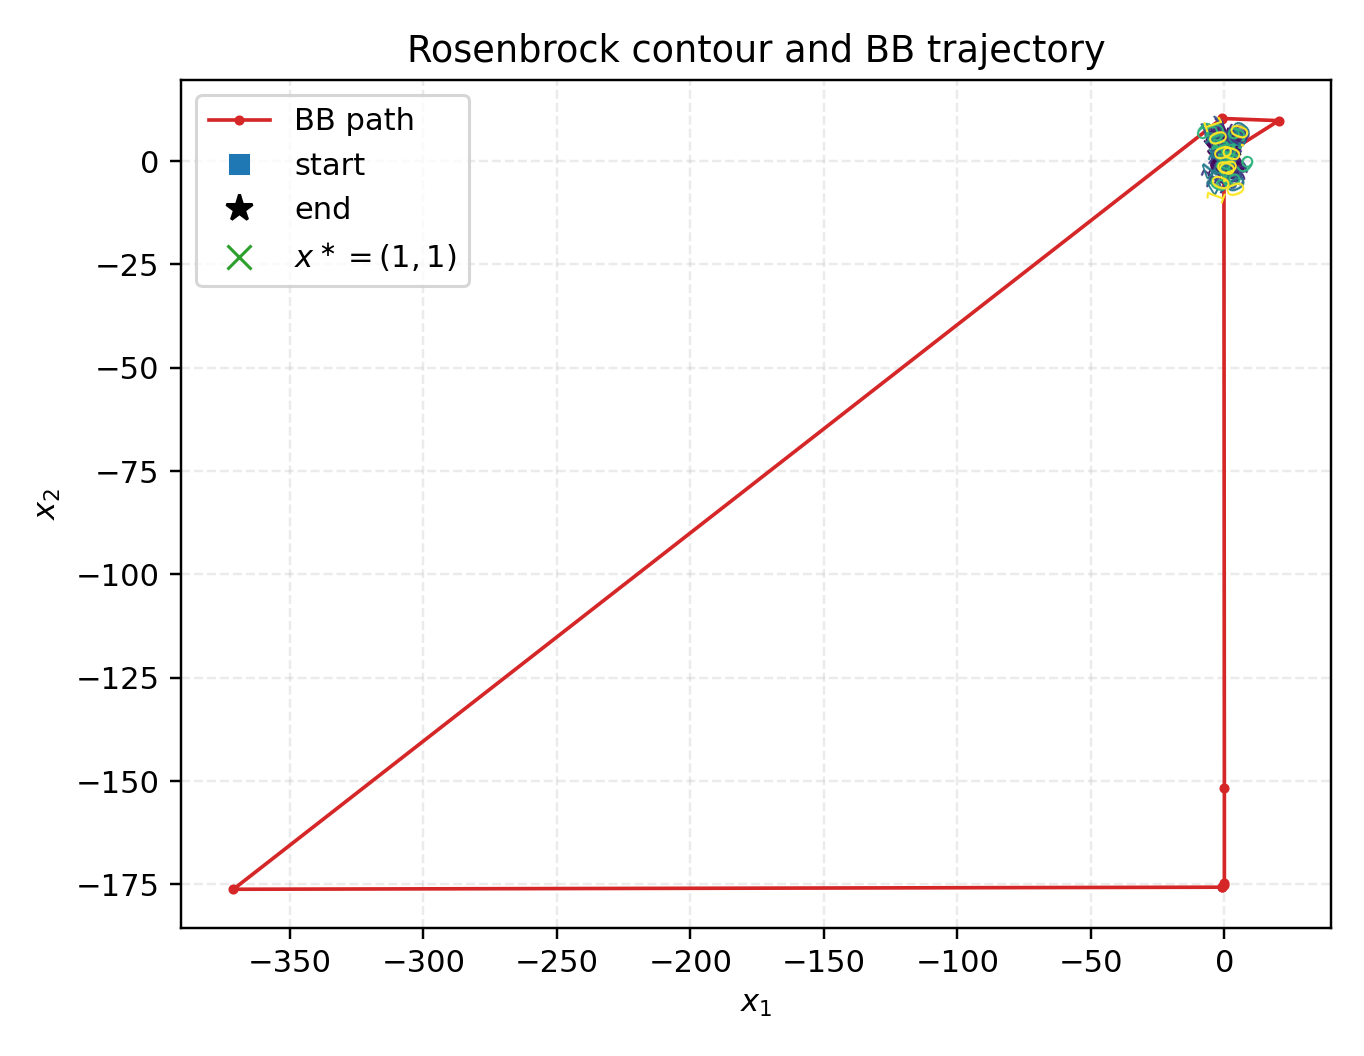
\includegraphics[width=\linewidth]{picture/work3_rosenbrock_bb_contour}
  \caption{Rosenbrock 等高线与 BB 迭代轨迹}
\end{subfigure}
\hfill
\begin{subfigure}{0.48\linewidth}
  \centering
  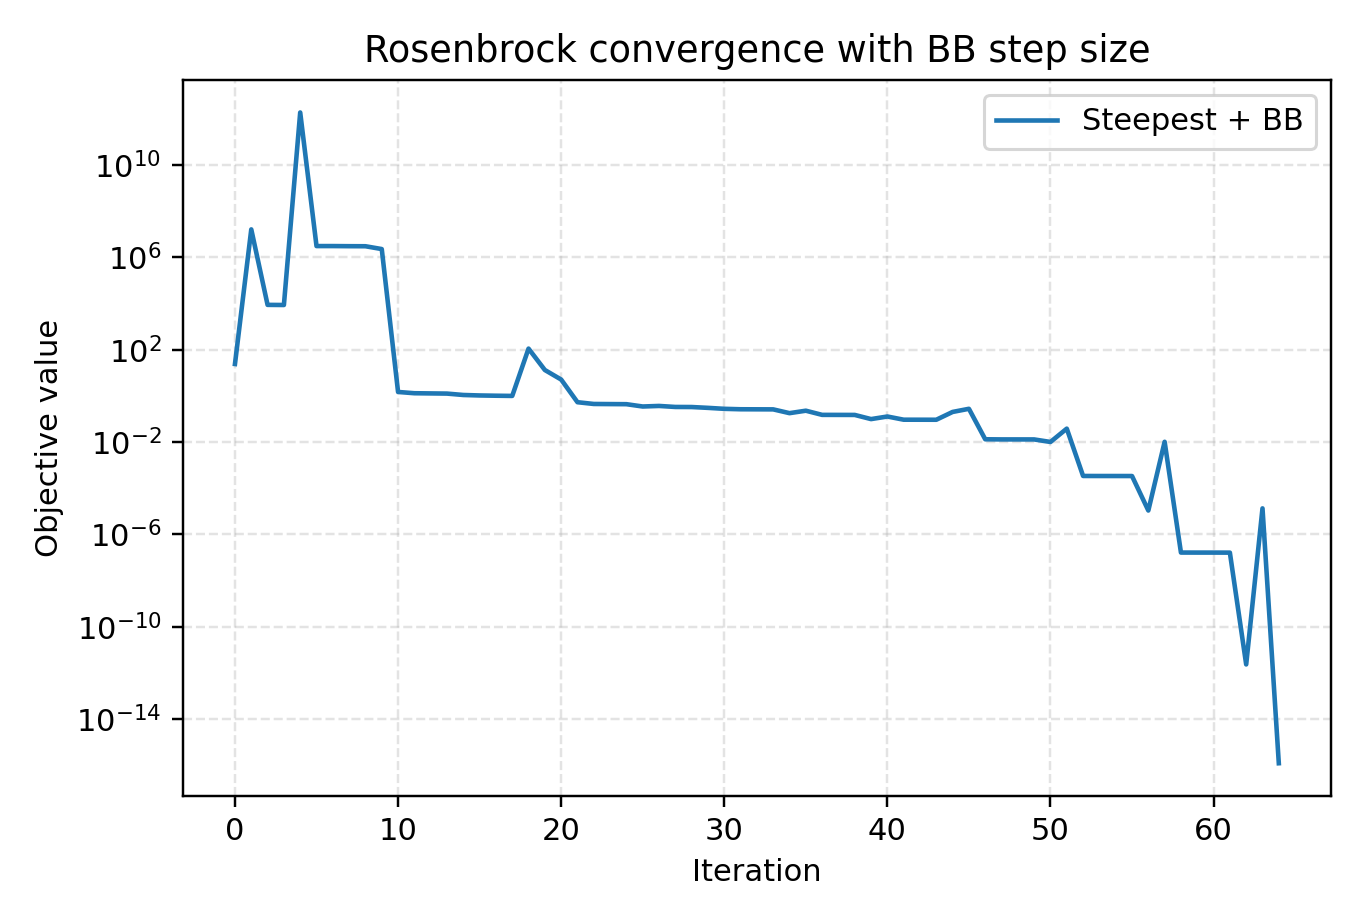
\includegraphics[width=\linewidth]{picture/work3_rosenbrock_bb_curve}
  \caption{Rosenbrock 目标函数值收敛曲线}
\end{subfigure}
\caption{BB 步长在 Rosenbrock 问题上的优化过程。}
\label{fig:work3_rosen}
\end{figure}

从图 \ref{fig:work3_rosen} 可以看到，BB 步长在谷底附近仍存在一定摆动，但相比固定步长最速下降法，收敛速度明显提升，能够在较少迭代内达到较高精度。

\subsection{Armijo + BFGC/FR（Powell 奇异函数）}
\begin{table}[H]
\centering
\caption{Powell 奇异函数上的算法对比}
\label{tab:work3_powell}
\begin{tabular}{lcccc}
\toprule
方法 & 迭代次数 & $f^\ast$ & 是否收敛 & $\|\nabla f(x^\ast)\|$ \\
\midrule
BFGC + Armijo & 29 & $3.2600\times 10^{-10}$ & 是 & $7.3476\times 10^{-7}$ \\
FR + Armijo & 115 & $4.7300\times 10^{-12}$ & 是 & $6.5085\times 10^{-7}$ \\
\bottomrule
\end{tabular}
\end{table}

\begin{figure}[H]
\centering
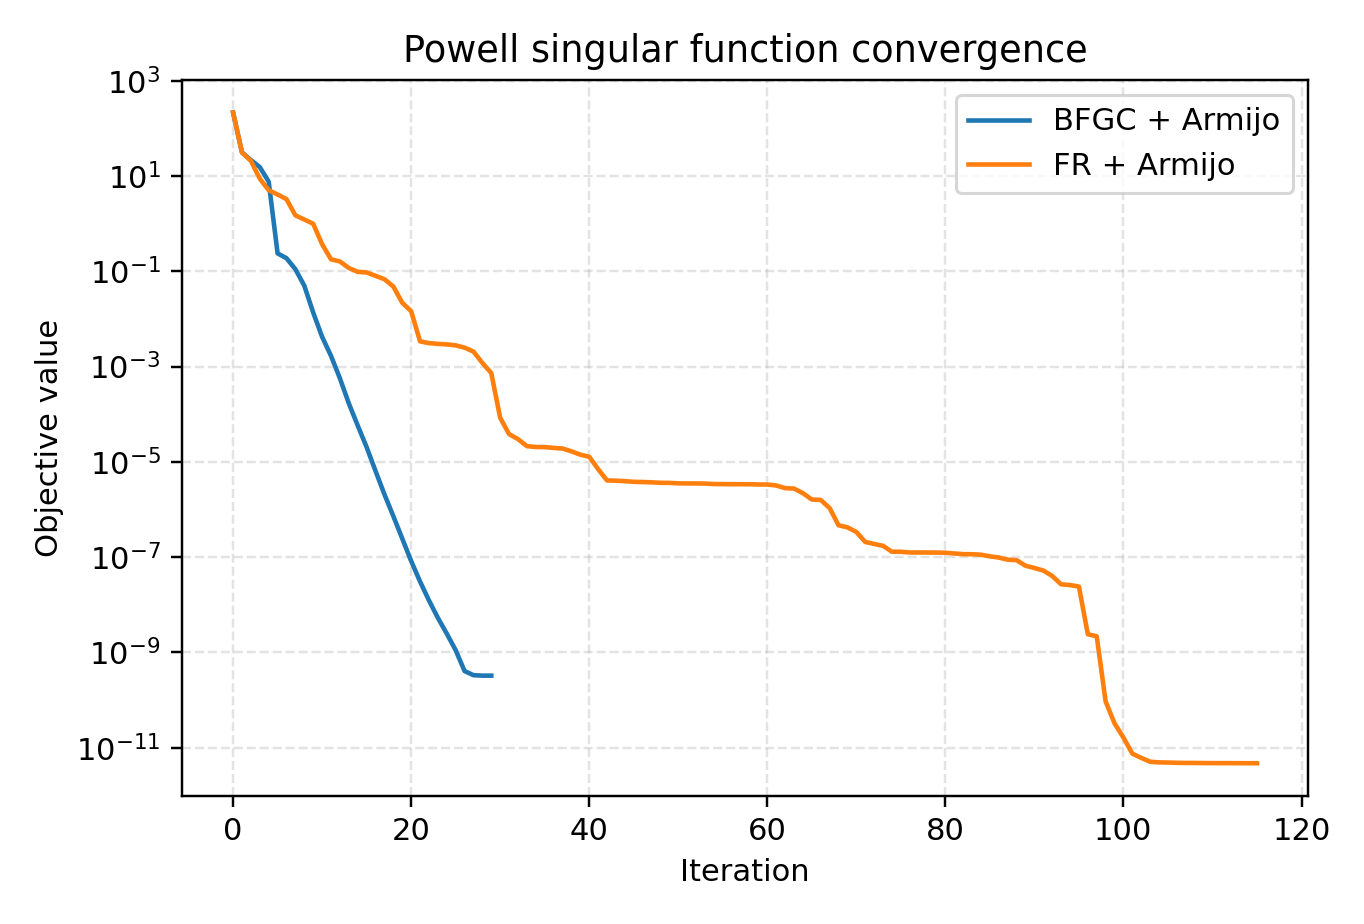
\includegraphics[width=0.72\linewidth]{picture/work3_powell_armijo_curve}
\caption{Powell 奇异函数上，BFGC 与 FR 在 Armijo 步长搜索下的收敛曲线。}
\label{fig:work3_powell_curve}
\end{figure}

由表 \ref{tab:work3_powell} 和图 \ref{fig:work3_powell_curve} 可见：
BFGC 迭代次数更少，表现出拟牛顿法利用曲率信息的优势；
FR 迭代次数较多，但最终函数值更低，说明在该问题上其后期下降能力也较强。

\end{document}
